\chapter{}

Tomaz nasceu em quatro de fevereiro de mil novecentos e setenta e três, de parto normal.
A experiência de dar à luz foi para mim transcendental, indescritível e intransferível.
Por mais que minha mãe, parturiente de cinco filhos como eu própria seria, descrevesse em detalhes o que era e como era, nada me preparou para o que eu senti.
Os movimentos do meu corpo, o instante do nascimento, a dor que me rasgou como um raio e me lançou para além de mim, desaparecendo em seguida como por encanto quando o choro do meu filho me trouxe de volta àquela sala, tudo pareceu obedecer a uma força ancestral, sobre-humana e poderosa que me fez atravessar por um brevíssimo instante o limiar da eternidade.
Quando o puseram sobre mim, abracei-o, chorando.

\begin{figure}
\centering
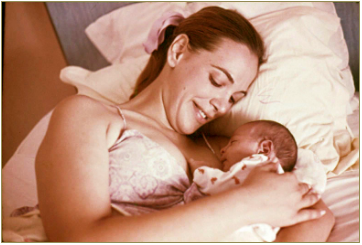
\includegraphics[width=0.8\linewidth]{24/tomaz-primeiras-horas.png}
\caption{Tomaz, nas primeiras horas de vida.}
\end{figure}

Quando meu filho foi trazido ao quarto, poucas horas depois, observando-lhe a fisionomia severa e a testinha sempre franzida sabe-se lá por que espécie de preocupação, mamãe opinou que talvez fosse mais adequado oferecer-lhe um charuto ao invés da chupeta.
Era evidente que o rapazinho não combinava com rendas, touquinhas e \textit{bilu-bilus}.
Era um machinho atento, determinado e incisivo.
Durante os três dias que passei na maternidade, mal ele acordava as enfermeiras traziam-no correndo até mim, porque seu choro não passava pelo estágio prenunciador dos resmungos.
Já eclodia a plenos pulmões, pondo todo o berçário em alvoroço.

Quando saí da maternidade, fiquei ainda um mês me recuperando em Araraquara, para enfrentar a longa viagem de volta a Campo Grande.
O avô Mathias, ao anoitecer, deitava Tomaz ao seu lado na cama e entretinha-se com ele em longas conversas.
O garotinho parecia ouvi-lo quieto, concentrado, sempre de cenho franzido.

\textit{``-- Vejam só''}, dizia meu pai, fascinado,  \textit{``tenho a impressão de que esse menino faz força para entender o que eu falo!''}

Observando as famílias hoje em dia, fica evidente o resultado da pressão da sociedade para que os parceiros masculinos se envolvam mais com a gestação, o parto e a educação dos filhos.
Naquele tempo, no tocante aos dois primeiros estágios, a maioria dos homens não tinha a menor idéia de como isso podia ser feito.
Um filho só entrava na área de competência de um homem quando fosse capaz de chamá-lo de papai.
E olhe lá! A maioria ficava orgulhosa do feito, sobretudo se fosse menino, mas a paternidade era um conceito a ser maturado e assimilado ao longo dos anos.
Bebês eram assunto para as mães.
Os homens aprendiam que era assim e as mulheres também.
Daí que a primeira impressão do Paulo, no dia do nascimento do Tomaz, foi a de ter sido uma presença dispensável.
Segundo ele, todas as atenções se voltaram para mim e para o nenê e ninguém se preocupou em saber como ele estava se sentindo.
Talvez por isso, logo após ter certeza de que estávamos bem e dormindo, extenuados, ele sumiu e caminhou por longas horas sozinho, tentando internalizar a experiência de se tornar pai.
Voltou ao amanhecer e só então entregou-se à tarefa de comunicar o evento a parentes e amigos e a receber parabéns por ter gerado um molecão que era a cara dele e de ``saco preto'', ainda por cima, para inveja dos cunhados que até então só tinham conseguido fazer meninas.
Na verdade, apenas João e Paulinho, anos mais tarde, teriam filhos homens.
Depois, em companhia do sogro, cumpriu o ritual de registrar o menino, tarefa a que meu pai atribuía extrema importância.
Todas as certidões dos nossos filhos contaram com seu infalível testemunho.

Só lamento que por uma incompreensível atitude minha, pela qual me amaldiçoarei para sempre, dispensei dos nomes das crianças o meu nome de família.
Tenho certeza de que causei ao meu pai, com esse estúpido menosprezo, uma grande decepção.

Ao final de fevereiro, voltamos para casa.
Éramos uma família agora e a responsabilidade por aquela sensação era daquela trouxinha de pano arrulhante que eu carregava nos braços.

As coisas na fazenda não iam bem.
Paulo continuava viajando para lá às segundas-feiras e voltando aos sábados.
Eu me devotava ao bebê, inteiramente.
Não havia espaço para mais preocupações.
Paulo sentia e me poupava.
Ao fim de um mês, Tomaz contraiu uma infecção de garganta que acabou contaminando os ouvidos e começamos, ele e eu a percorrer um calvário que se estenderia por quase dois meses.
Ele chorava desesperadamente, dia e noite, de dor.
Nos fins de semana, Paulo chegava tão cansado que mesmo com toda boa vontade em me ajudar, tinha dificuldade em se manter acordado.
Eu não confiava nos médicos da cidade, nosso menino teve que tomar um monte de injeções para vencer a infecção e, para finalizar, recebeu drenos nos ouvidos, porque já não era possível continuar puncionando seus tímpanos.

Finalmente uma manhã, após muitas semanas de noites mal dormidas, dei-me conta, ao acordar, de que Tomaz dormira a noite inteirinha.
Quando corri para o berço, ansiosa, ele levantou os bracinhos e sorriu, feliz.
Caí no choro.

Horas depois, Lenita, uma amiga do prédio, ao dar comigo ainda em camisola, despenteada e agarrada ao meu filho, passou-me uma descompostura em regra:.

\textit{``-- Chega! Não dá mais para ver você assim! Não sei como teu pobre marido aguenta! Você parece uma paraguaia `véia', daquelas que ficam na porta da choupana chacoalhando menino no colo o dia inteiro.
Bote essa criança no carrinho, vá vestir uma roupa, pentear o cabelo, passar um batom e já para a rua! Vamos passear!''}

\textit{``--De que jeito?''}, perguntei, \textit{``Tomaz é muito pequeno e mal sarou!''}

\textit{``-- Do mesmo jeito que a minha filha, que é apenas um mês mais velha que seu filho, me acompanha para todo lado e vai até no boteco comigo e com meu marido, quando vamos tomar chope.
Ou será que a sua vida acabou porque você virou mãe?''}

Foi uma pancada merecida.
De repente, dei-me conta de que Tomaz se transformara no pretexto para que eu me ausentasse da vida, fugisse dos problemas e pior, me erigisse em vítima.
Era Paulo quem necessitava de ajuda agora e eu precisava me inteirar do que acontecia e de como ele estava lidando com a situação.
Foi então que mergulhamos nos primeiros conflitos sérios do nosso casamento.

Pela vida toda mamãe se jactou do fato de que jamais um cobrador bateu à nossa porta.
Meu pai tinha o perfil acabado do provedor.
Em razão disso, nossa família pode ter passado por problemas sérios, sim, mas nenhum que ameaçasse nem de leve nossa segurança material.
Eu não sabia o que era viver com dívidas.
O plano que Paulo tinha em mente era conseguir empréstimos-ponte nos bancos para sustentar a fazenda até que o IBC retomasse as liberações ou, na pior das hipóteses, até a colheita, quando então saldaríamos todos os compromissos.
Imaginando a quanto montariam essas cifras ao final do tempo que ainda tínhamos pela frente, juros se multiplicando, a idéia me pareceu absolutamente inaceitável.
Era sacar sobre o futuro e nos condenar a uma espécie de escravidão da qual só Deus sabia quando iríamos nos livrar.
Paulo, que nesse terreno a vida toda lidara com o imponderável, não via as coisas dessa maneira e achava que eu estava me portando como uma tola mimada, sem noção da realidade.
Hoje, admito que ele tinha razão, sob certos aspectos, porque a minha proverbial incapacidade de pensar em números, tornava difícil, para mim, cotejar as dívidas com o potencial de ganhos do cafezal.


\begin{figure}
\centering
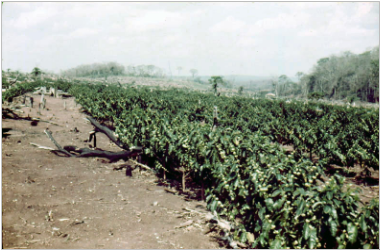
\includegraphics[width=0.8\linewidth]{24/cafezal-em-flor.png}
\caption{O cafezal em flor da Santa Teresa.}
\end{figure}


Além do mais, não se podia jogar todo o trabalho feito para o alto e desistir de tudo assim, sem mais.
Mas eu estava muito apreensiva e convencida de que faltava ao meu marido a presença de alguém experiente que o ajudasse a encontrar uma saída.
Como não podia contar com o pai dele, pensava no meu.
A esta altura, também, o tempo de afastamento que eu obtivera do meu trabalho em Araraquara estava prestes a esgotar-se e eu tinha que me decidir entre pedir demissão ou voltar para reassumi-lo.
Naquelas circunstâncias, abrir mão de um salário me parecia o cúmulo da irresponsabilidade, mesmo que ele não fosse grande coisa.
Comecei a insistir na ideia de voltar para São Paulo.
Paulo acabou cedendo, mas nunca me perdoou.
Essa não seria a primeira vez em que, ao invés de apoiá-lo na decisão de ir em frente, eu optaria por bater em retirada.

Ao longo da nossa vida em comum, a exigência do Paulo por adesão incondicional às suas iniciativas foi para mim fonte de angústia permanente.
Por um lado, conhecendo sua crônica insegurança e sua permanente ansiedade, eu sentia que lhe devia esse apoio.
Por outro, porém, essa inclinação esbarrava em dois obstáculos fortemente entrelaçados: o meu complexo ainda não resolvido de não me sentir capaz de assegurar minha própria independência material e a minha preocupação com a segurança dos filhos.
 Por longo tempo alimentei a crença de que a ousadia do Paulo em encetar grandes negócios ou, pelo menos, negócios sempre acima dos nossos parcos recursos, tinha relação com aquela ancestral ``psicose da redenção'' que afetava a família dele e que lhe teria sido introjetada pela influência direta de José Ignácio e Roberto.
Essa suspeita o enfurecia sobremaneira.
Só muito tempo depois aprendi que, nele, tais iniciativas eram principalmente uma espécie de super-reação ao medo permanente que sentia de não dar conta da vida, somado à busca de reconhecimento, fatores responsáveis por levá-lo a gigantescos esforços de superação em empreitadas sempre acima da capacidade do comum das pessoas.

Voltamos para Araraquara e eu retomei minhas funções de professora.
Por algum tempo, Paulo ainda permaneceu lutando para manter a fazenda.
O café estava lindo, florido e a expectativa de uma excepcional colheita lhe dava razão.
